\documentclass[12pt,a4paper]{article}
%%% Работа с русским языком
\usepackage{cmap}					% поиск в PDF
\usepackage{mathtext} 				% русские буквы в формулах
\usepackage[T2A]{fontenc}			% кодировка
\usepackage[utf8]{inputenc}			% кодировка исходного текста
\usepackage[english,russian]{babel}	% локализация и переносы

%%% Дополнительная работа с математикой
\usepackage{amsmath,amsfonts,amssymb,amsthm,mathtools} % AMS
\usepackage{icomma}
\usepackage{physics}
\usepackage{multicol}
\usepackage{bm}
\usepackage{mathrsfs}
\usepackage{verbatim}

%%% Номера формул
%\mathtoolsset{showonlyrefs=true} 
%\usepackage{leqno} 

%%% Свои команды
\DeclareMathOperator{\sgn}{sgn}

\usepackage{csquotes} 
\usepackage[backend=biber,style=authoryear,language=auto]{biblatex}


%%% Работа с графикой
\usepackage{graphicx}
\graphicspath{{images/}}  
\setlength\fboxsep{3pt} 
\setlength\fboxrule{1pt} 
\usepackage{wrapfig} 
\usepackage{tikz}
\usepackage{pgfplots}
\usepackage{pgfplotstable}
\usepgfplotslibrary{polar}
\pgfplotsset{compat=1.18} 

%%% Работа с таблицами
\usepackage{array,tabularx,tabulary,booktabs}
\usepackage{longtable}  
\usepackage{multirow} 
\usepackage{caption2}[2008/03/29]
\usepackage{soul} 

%%% Теоремы
\theoremstyle{plain} 
\newtheorem{theorem}{Th}[section]
\newtheorem{proposition}[theorem]{Proposition}
 
\theoremstyle{definition} 
\newtheorem{corollary}{Corollary}[theorem]
\newtheorem{problem}{Problem}[section]
\newtheorem{definition}{Def}[section]
 
\theoremstyle{remark} 
\newtheorem*{nonum}{Solution}

%%% Программирование
\usepackage{etoolbox} 

%%% Гиперссылки
\usepackage{hyperref}

\usetikzlibrary{knots}
\usepackage{tcolorbox}

%%% Страница
\usepackage{geometry} 
	\geometry{top=20mm, bottom=20mm, left=15mm, right=20mm}

\usepackage{setspace} 

\usepackage{lastpage} 
\usepackage{amssymb}
\usepackage{xcolor}
\DeclareMathOperator{\Ker}{Ker}
\DeclareMathOperator{\qdim}{qdim}

\addbibresource{../source.bib}
\begin{document}

\begin{center}
    \Large \textbf{Полиномы Хованова-Рожанского} \\[1em]
    \small
    Московский Физико-Технический Институт \\[0.5em]
    Лаборатория Математической и Теоретической Физики
\end{center}

\small
\begin{flushright}
\begin{tabular}{c c}
\textbf{Авторы:} & \textbf{Научные руководители:} \\[0.5em]
Артем Новохатний & Елена Ланина \\
Екатерина Цыганкова & Радомир Степанов \\
Эльдар Мифтахов & \\
\end{tabular}

\vspace{1em}

\today
\end{flushright}
\normalsize
\vspace{2em}


\tableofcontents
\vspace{2em}

\section{Полиномы Джонса}

\subsection{Вопросы}
\begin{itemize}
    \item  Можно ли из скобки Кауффмана получить полином Кауффмана?
    \item  Какие допаксиомы нужны, чтобы определить полином Джонса через скейн-соотношение на перекрестки?
    \item  Добавить другие степени в левой части скейн-соотношения. Будет ли это ещё инвариантом?
    \item Джонс нормируется на аннот. Как нормировать Ховановых?
\end{itemize}

\section{Khovanov polynomial}
The statesum form (equation ...) of the Kauffman bracket allows the following interpretation. Let us consider each circle in a completely smoothed diagram $\alpha \in \{0, 1\}^\chi$ as a graded vector space $V$ with grading $\{+, -\}$.  If $\alpha$ consists of $n$ circles, we associate it with $V^{\otimes n}$. Then we group complete smoothings according to the number of 1-resolutions $\gamma$ and consider these groups as a direct sum of vector spaces $V_\gamma = \bigoplus\limits_{\alpha(\gamma)} V^{\otimes n(\alpha)}$. The dimension of the resulting space is exactly equal to the $(-q)^\gamma$ prefactor in statesum.


\subsection{Example: positive Hopf link}

\begin{wrapfigure}{r}{0.2\textwidth}
  \begin{center}
    \begin{minipage}{\linewidth}
      \resizebox{\linewidth}{!}{\begin{tikzpicture}
  \begin{knot}[
    clip width=5,
    flip crossing/.list={1}
  ]
    % первая окружность по дугам
    \strand[line width=3pt,->,black] 
      (0,0) arc[start angle=0,end angle=360,radius=1];
    
    % вторая окружность по дугам
    \strand[line width=3pt,<-,black] 
      (-1,0) arc[start angle=0,end angle=360,radius=-1];
  \end{knot}
\end{tikzpicture}}
  \end{minipage} 
    $n_{+} = 2$

  $n_{-} = 0$
  \end{center}
\end{wrapfigure}

\[
\mathcal{H}^0 = \Ker d_{01} = \langle v_- \otimes v_-, v_- \times v_+ - v_+ \times v_-\rangle \{2\} ~~ \Rightarrow ~~ \qdim\mathcal{H}^0 = 1 + q^2
\]

\[
\mathcal{H}^1 = \Ker d_{12}/\Im d_{01} = \frac{\langle v_{+(1)} + v_{+(2)}, v_{-(1)} + v_{-(2)}\rangle}{\langle v_{+(1)} + v_{+(2)}, v_{-(1)} + v_{-(2)}\rangle}\{3\} ~~ \Rightarrow ~~ \qdim\mathcal{H}^1 = 0
\]

\[
\mathcal{H}^2 = V/\Im d_{12} = (V/\langle v_- \otimes v_-, v_- \times v_+ + v_+ \times v_-\rangle)\{4\} ~~ \Rightarrow ~~ \qdim\mathcal{H}^1 =  q^4 + q^6
\]

\[\boxed{Kh(\begin{minipage}{0.06\linewidth}
      \resizebox{\linewidth}{!}{\begin{tikzpicture}
  \begin{knot}[
    clip width=5,
    flip crossing/.list={1}
  ]
    % первая окружность по дугам
    \strand[line width=3pt,->,black] 
      (0,0) arc[start angle=0,end angle=360,radius=1];
    
    % вторая окружность по дугам
    \strand[line width=3pt,<-,black] 
      (-1,0) arc[start angle=0,end angle=360,radius=-1];
  \end{knot}
\end{tikzpicture}}
  \end{minipage} ) = 1 + q^2 + t^2 q^4 + t^2 q^6}
\]
\begin{figure}[h]
    \begin{center}
    \begin{tikzpicture}
    \node at (-0.5, 0) {0};
    \draw[->] (0,0) -- (1,0) node[midway, above] {$d_{00}$};

    \node[inner sep=0pt] at (2.5,0) {
    \resizebox{2cm}{!}{
        \begin{tikzpicture}
            \begin{knot}[clip width=5]
                \strand[line width=2pt, black]
                    (-0.2, 0.7) to[out=90,in=90,looseness=1]
                    (-1.5, 0) to[out=-90,in=-90,looseness=1]
                    (-0.2, -0.7) to[out=90,in=-90,looseness=1]
                    (-0.7, 0) to[out=90,in=-90,looseness=1] (-0.2, 0.7);

                \strand[line width=2pt, black]
                    (0.2, 0.7) to[out=90,in=90,looseness=1]
                    (1.5, 0) to[out=-90,in=-90,looseness=1]
                    (0.2, -0.7) to[out=90,in=-90,looseness=1]
                    (0.7, 0) to[out=90,in=-90,looseness=1] (0.2, 0.7);
            \end{knot}
        \end{tikzpicture}
    }
    };

    \draw[->] (4,0.5) -- (5,1.5) 
    node[pos=0.25, right = 3pt] {$d_{\bigstar 0}$}
    node[pos=0.5, left = 3pt] {$m$};
    \draw[->] (4,-0.5) -- (5,-1.5) 
    node[pos=0.25, right = 3pt] {$d_{0 \bigstar}$}
    node[pos=0.5, left = 3pt] {$m$};

    \node[inner sep=0pt] at (6.5, 1.5) {
    \resizebox{2cm}{!}{
        \begin{tikzpicture}
            \begin{knot}[clip width=5]
                \strand[line width=2pt, black]
                    (0, 0.8) to[out=180,in=0,looseness=1]
                    (-0.7, 1) to[out=180,in=180,looseness=1]
                    (-0.7, -1) to[out=0,in=-90,looseness=1]
                    (-0.2, -0.7) to[out=90,in=180,looseness=1]
                    (0, 0.4) to[out=0,in=90,looseness=1]
                    (0.2, -0.7) to[out=-90,in=180,looseness=1]
                    (0.7, -1) to[out=0,in=0,looseness=1]
                    (0.7, 1) to[out=180,in=0,looseness=1] (0, 0.8);
            \end{knot}
        \end{tikzpicture}
    }
    };

    \node[inner sep=0pt] at (6.5, -1.5) {
    \resizebox{2cm}{!}{
        \begin{tikzpicture}
            \begin{knot}[clip width=5]
                \strand[line width=2pt, black]
                    (0, -0.8) to[out=180,in=0,looseness=1]
                    (-0.7, -1) to[out=180,in=180,looseness=1]
                    (-0.7, 1) to[out=0,in=90,looseness=1]
                    (-0.2, 0.7) to[out=-90,in=180,looseness=1]
                    (0, -0.4) to[out=0,in=-90,looseness=1]
                    (0.2, 0.7) to[out=90,in=180,looseness=1]
                    (0.7, 1) to[out=0,in=0,looseness=1]
                    (0.7, -1) to[out=180,in=0,looseness=1] (0, -0.8);
            \end{knot}
        \end{tikzpicture}
    }
    };

    \draw[->] (8,1.5) -- (9,0.5) 
    node[pos=0.75, left = 3pt] {$d_{1 \bigstar}$}
    node[pos=0.25, right = 3pt] {$-\Delta$};
    \draw[->] (8,-1.5) -- (9,-0.5) 
    node[pos=0.75, left = 3pt] {$d_{\bigstar 1}$}
    node[pos=0.25, right = 3pt] {$\Delta$};

    \node[inner sep=0pt] at (10.5, 0) {
    \resizebox{2cm}{!}{
        \begin{tikzpicture}
            \begin{knot}[clip width=5]
                \strand[line width=2pt, black]
                    (0, 0.8) to[out=180,in=0,looseness=1]
                    (-0.7, 1) to[out=180,in=180,looseness=1]
                    (-0.7, -1) to[out=0,in=180,looseness=1]
                    (0, -0.8) to[out=0,in=180,looseness=1]
                    (0.7, -1) to[out=0,in=0,looseness=1]
                    (0.7, 1) to[out=180,in=0,looseness=1](0, 0.8);
                \strand[line width=2pt, black] 
                    (0,0) circle[radius=0.5cm];
            \end{knot}
        \end{tikzpicture}
    }
    };

    \draw[->] (12,0) -- (13,0) node[midway, above] {$d_{11}$};
    \node at (13.5, 0) {0};


    \draw[blue] (3.7,2) rectangle (5.3,-2);
    \draw[->, blue] (4,-2.7) -- (5,-2.7) node[midway, above, blue]{$d_{01}$};

    \draw[blue] (7.7,2) rectangle (9.3,-2);
    \draw[->, blue] (8,-2.7) -- (9,-2.7) node[midway, above, blue]{$d_{12}$};

    \node at (2.5, -2.7) {\scriptsize $V_0 = V^{\otimes 2} \{0\} \textcolor{red}{\{2\}}$};
    \node at (6.5, -2.7) {\scriptsize $V_1 = V^{\oplus 2} \{1\} \textcolor{red}{\{2\}}$};
    \node at (10.5, -2.7) {\scriptsize $V_2 = V^{\otimes 2} \{2\} \textcolor{red}{\{2\}}$};

\end{tikzpicture}
    \caption{Positive Hopf link Khovanov complex. $\textcolor{red}{\{n_{+}-2n_{-}\} = \{2\}}$ -- common degree shift}
    \end{center}
\end{figure}

\section{HOMFLY polynomial}
\subsection{HOMFLY definition by skein-relation}

\subsection{HOMFLY definition by $\mathcal{R}$-matrices braid group representation}

The closure of a braid is the link obtained from the braid by connecting upper
ends and lower ends respectively as shown in Fig. .... The following theorem
assures us that such an expression always exists.
\begin{tcolorbox}
\begin{theorem}\label{thm:Alexander}
   (Alexander). Any (oriented) link is isotopic to the closure of some
braid (with downward orientation).  
\end{theorem}
\end{tcolorbox} 

However, as our intuition suggests, knots and braids have similar but not identical natures, so a single knot can be represented by a set of different braids (see example in Fig. ...). Nevertheless, this equivalence relation can be reformulated in terms of braid algebra operations, as stated by the following theorem.
\begin{tcolorbox}
\begin{theorem}\label{thm:Alexander}
   (Markov).  Let $b$ and $b'$ be two braids, and $L$ and $L'$ their closures.
Then, $L$ is isotopic to $L'$ as oriented links if and only if $b$ is related to $b'$ by a
sequence of the following MI and MII moves.

\begin{center}
\begin{tabular}{c c}
\textbf{MI:} & \textbf{MII:} \\
$ab \longleftrightarrow ba$ & $b \sigma_n \longleftrightarrow b \longleftrightarrow b \sigma_n^{-1}$ \\[2mm]  
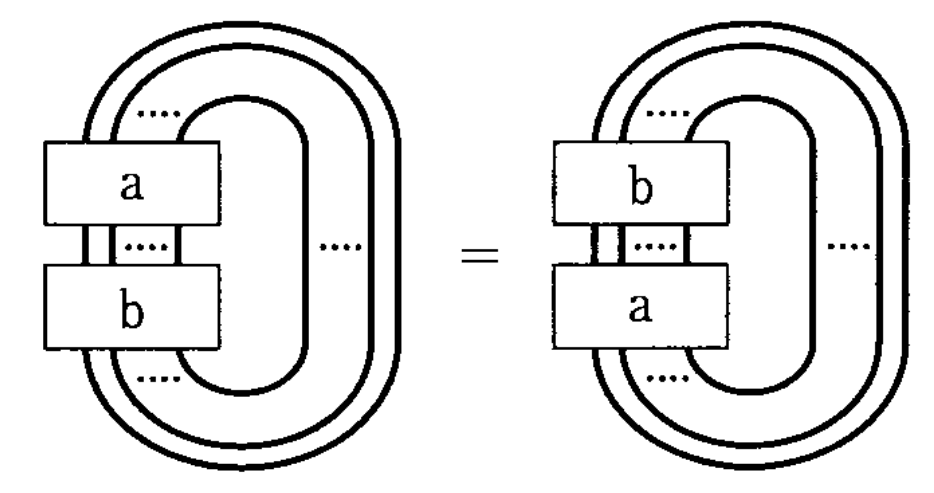
\includegraphics[height=3cm]{../img/MI.png} &
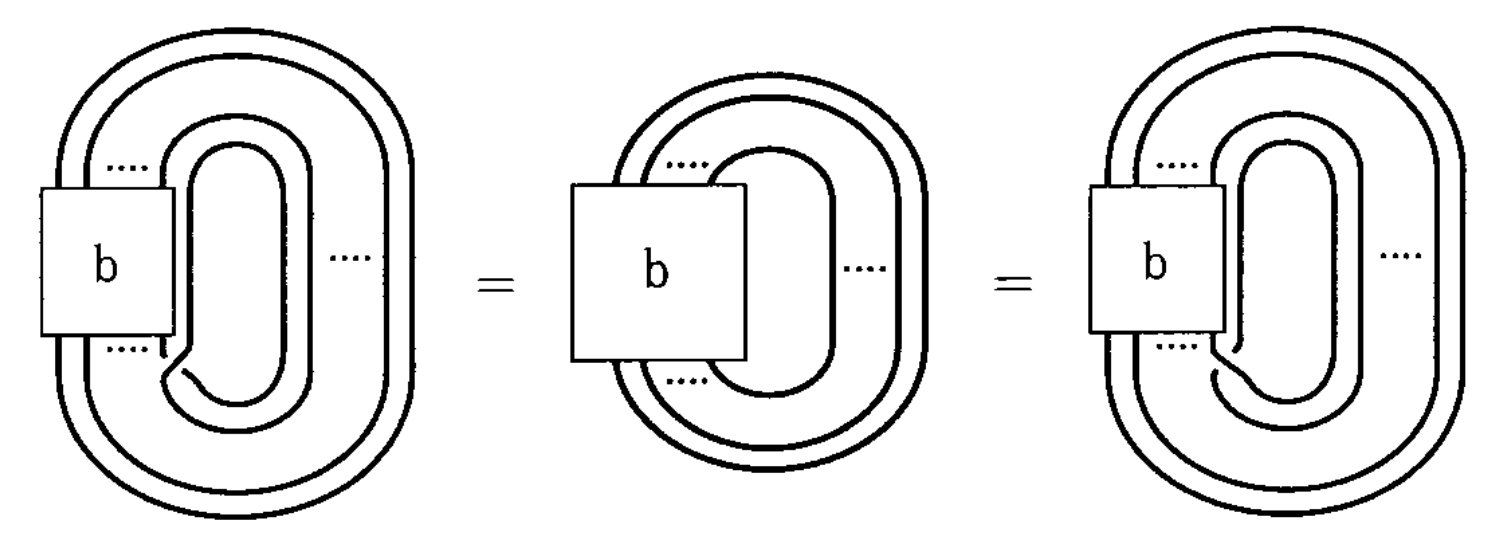
\includegraphics[height=3cm]{../img/MII.png}
\end{tabular}
\end{center}

\end{theorem}
\end{tcolorbox} 

\subsubsection{$\mathcal{R}$-matrices}
\begin{tcolorbox}
\begin{definition}
    Let $\mathfrak{g}$ be a simple finite-dimensional Lie algebra over $\mathbb{C}$. 
The \emph{quantized universal enveloping algebra} $U_q(\mathfrak{g})$ is an associative algebra over $\mathbb{C}(q)$ generated by elements
\[
\{ E_i, F_i, K_i^{\pm 1} \mid i = 1, \dots, \mathrm{rank}(\mathfrak{g}) \},\] 
where $E_i$ and $F_i$ -- simple positive and negative roots, respectively; $K_i = q^{h_i}$ -- quantization of the Cartan element $h_i$. $A = (a_{ij})_{ij}$ -- Cartan matrix.

Commutation relations:




\end{definition}
\end{tcolorbox}

\printbibliography

\end{document}